\documentclass{article}
\usepackage[utf8]{inputenc}
\usepackage{indentfirst}
\usepackage{amsmath}
\usepackage{amsthm}
\usepackage{graphicx}
\usepackage{float}
\title{RL Crash Course + Some Thoughts}
\author{Ding (Eric) Ding}
\date{November 2022}
\begin{document}

\maketitle

\section{Introduction}
    In this Project, I followed OpenAI deep reinforcement learning course, and used Spinning Up for exercises and experiments.

\section{What's Omitted}
    Regularization, Observation normalization

\section{Key Concepts}
    The main characters of RL are the agent and the environment. The environment is the world that the agent lives in and interacts with. At every step of interaction, the agent sees a (possibly partial) observation of the state of the world, and then decides on an action to take. The environment changes when the agent acts on it, but may also change on its own.
    \begin{figure}[H]
        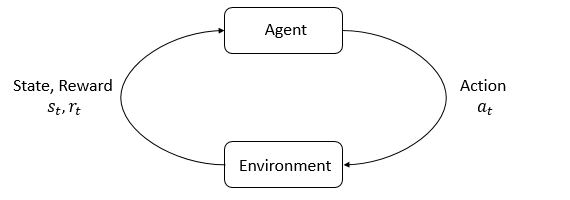
\includegraphics[width=\linewidth]{rl_diagram_transparent_bg.png}
        \caption{RL framework}
        \label{fig:rl}
      \end{figure}

    The agent also perceives a reward signal from the environment, a number that tells it how good or bad the current world state is. The goal of the agent is to maximize its cumulative reward, called return. Reinforcement learning methods are ways that the agent can learn behaviors to achieve its goal.

    States and observations: represented by matrix

    Action Spaces: the set of all valid actions. Discrete / continuous.

    Policies: a rule used by an agent to decide what actions to take. Deterministic: $a_t = \mu_{\theta}(s_t)$. Stochastic: $a_t \sim \pi_{\theta}(\cdot | s_t)$. In deep RL, we deal with parametrized policies, with parameters that can be adjusted by optimization. 
    
    Stochastic policies: categorical policies in discrete action space and diagonal gaussian policies in continuous action spaces. Two key computations: sampling actions from the policy, and compute log likelihoods of particular actions.

    Trajectory: A sequence of states and actions in the world. Can be deterministic or stochastic based on policy. 

    Reward and return: $r_t = R(s_t, a_t, s_{t+1})$. Maximize cumulative return $R(\tau)$. Finite-horizon undiscounted return: $R(\tau) = \Sigma_{t = 0} ^T r_t$. Infinite-horizon discounted return: $R(\tau) = \Sigma_{t =0} ^{\infty}\gamma^tr_t$

    The goal in RL is to select a policy which maximizes expected return when the agent acts according to it. The probability of a trajectory: 
    $$P(\tau | \pi) = \rho_0(s_0) \prod_{t = 0} ^{T - 1} \pi(a_t | s_t) P(s_{t+1}|s_t, a_t)$$
    The expected return is:
    $$
    J(\pi) = \int_\tau P(\tau | \pi) R(\tau) = E_{\tau \sim \pi} [R(\tau)]
    $$
    The central optimization problem in RL can then be expressed by
    $$
    \pi^* = \arg\max_\pi J(\pi)
    $$

    Value functions: it's useful to know the value of a state, which is the expected return if start in that state. 1) On-Policy Value Function $V^\pi(s)$, start in state $s$ and always acts according to policy $\pi$. 2) On-Policy Action-Value Function $Q^\pi(s, a)$, start in state $s$, take arbitrary action $a$, and then acts according to policy $\pi$. 3) Optimal Value Function $V^*(s)$, start in state $s$ and acts according to the optimal policy. 4) Optimal Action Value Function $Q^*(s, a)$. 

    The Optimal Q-Function and the Optimal Action: $a^*(s) = \arg\max_a Q^*(s, a)$

    Bellman Equations: 
    $$
      V^\pi(s) = E_{a \sim \pi, s' \sim P}[r(s,a) + \gamma V^\pi(s')]
    $$
    $$
      Q^\pi(s, a) = E_{s' \sim P} [r(s, a) + \gamma E_{a' \sim \pi}[Q^\pi(s', a')]]
    $$
    $$
      V^*(s ) = \max_a E_{s' \sim P} [r(s, a) + \gamma V^*(s')]
    $$
    $$
      Q^*(s, a) = E_{s' \sim P} [r(s, a) + \gamma \max_{a'} Q^*(s', a')]
    $$

    Advantage Function:
      $$
        A^\pi(s, a) = Q^\pi(s, a) - V^\pi(s)
      $$

\section{Kinds of RL Algorithm}
  \begin{figure}[H]
    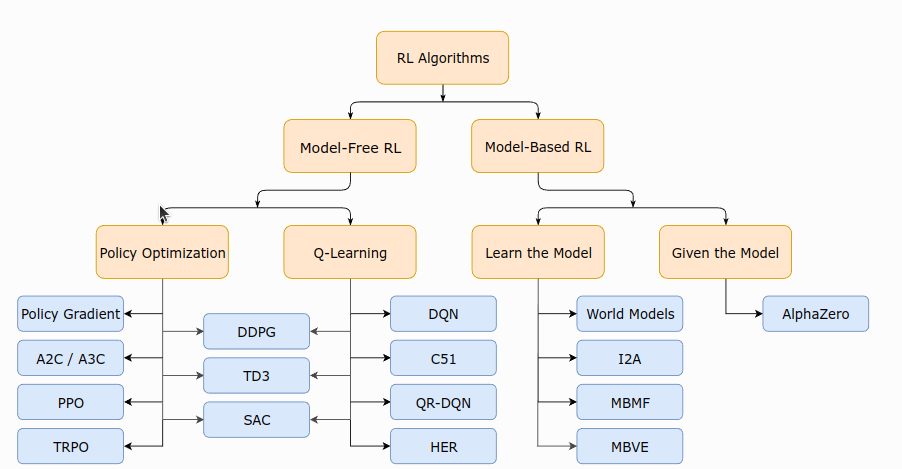
\includegraphics[width=\linewidth]{rlalg.png}
    \caption{RL Algorithm}
    \label{fig:ag}
  \end{figure}

\section{Ideas}
    \subsection{Observation}
      Fully observed environment vs. partially observed\
    \subsection{Action}
      Rule out certain actions in action space, can combine both stochastic and deterministic policy.
    \subsection{Value}\
      How to calculate value functions (future) and adjust policy accordingly (optimize)? 

\end{document}